\section{The pre-token floor binds vocabulary extension}
\label{sec:ceiling}

\paragraph{Pre-tokens bound tokens.} A byte-level BPE tokenizer first splits text $s$ with a regex into pre-tokens $P(s) = (p_1,\dots,p_m)$, then encodes each $p_i$ independently by applying merges in rank order. Since every non-empty pre-token yields at least one token, $|T(s)| \ge |P(s)|$, a bound \citet{regmi2026vowel} call the pre-tokenization ceiling. Vocabulary extension appends merges but leaves $P$ unchanged, so the same bound holds for every extended tokenizer. Strings registered as HuggingFace \emph{added tokens} bypass the bound (Appendix~\ref{app:released}).

\begin{observation}[Extension floor; a direct corollary of the bound of \citealp{regmi2026vowel}]
\label{prop:ceiling}
Let $T_K$ be any tokenizer obtained from $T$ by appending $K$ merges, for any $K$ and any set of merges regardless of training data, without changing its normalizer or pre-tokenizer and without added tokens. Then $|T_K(s)| \ge |P(s)|$ for every string $s$.
\end{observation}

To turn this into a floor on the premium, we divide by the English token count of the \emph{base} tokenizer. This step needs the extension to leave English unchanged. It does for \RI{}: every new merge outputs a token containing a code point in U+0900--U+097F, so no new merge can apply to English text, by the argument of Proposition~\ref{prop:lossless} with the regex left unchanged. The premium of \RI{} is therefore at least the pre-token floor of \S\ref{sec:audit}, for every $K$.

The bound is not loose for the regexes deployed today. In the Llama-3 and Qwen families, the word branch is \texttt{[\textasciicircum\textbackslash r\textbackslash n\textbackslash p\{L\}\textbackslash p\{N\}]?\textbackslash p\{L\}+}: a run of letters, optionally preceded by one non-letter. A Devanagari vowel sign is not a letter, so it ends the current run and is absorbed as the optional prefix of the next one. In Figure~\ref{fig:split}, the phrase \emph{nep\=alko sark\=ar} (``government of Nepal'') becomes six pre-tokens, four of which begin with a vowel sign that belongs to the \emph{previous} consonant. Under the repaired regex each word is one pre-token.

\begin{figure}[t]
\centering
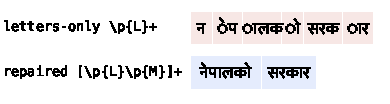
\includegraphics[width=0.95\columnwidth]{fig_split.pdf}
\caption{Pre-tokens of \emph{nep\=alko sark\=ar} (``government of Nepal'') under the letters-only regex of Llama-3 and Qwen and under the repaired regex. Dotted circles mark pre-tokens that begin with a dependent vowel sign.}
\label{fig:split}
\end{figure}

\paragraph{The floor, measured.} Table~\ref{tab:floor} gives the pre-token floor of Llama-3 and Qwen3 under their own letters-only regexes and under the repaired regex of each model. For both families the letters-only floor is about $2.2\times$, nearly three times the repaired floor ($2.77\times$ for Llama-3, $2.73\times$ for Qwen3), and above the premium of \texttt{o200k} ($1.61\times$).

\begin{table}[t]
\centering
\small
\begin{tabular}{lrrr}
\toprule
& Llama-3 & Qwen3 & \texttt{o200k} \\
\midrule
Current premium & 2.58 & 4.42 & 1.61 \\
Floor, letters-only regex & 2.19 & 2.17 & -- \\
Floor, repaired regex & 0.79 & 0.80 & 0.80 \\
\bottomrule
\end{tabular}
\caption{Nepali/English token premium on FLORES-200 devtest, and the pre-token floor under each regex (pre-tokens of Nepali / tokens of English): a lower bound on the premium of any vocabulary extension under that regex. Each model's floors use its own pattern (Qwen splits digits singly, Llama-3 in groups of up to three). Llama-3 and Qwen3 ship the letters-only regex; for \texttt{o200k}, which ships a mark-aware regex, the floor is under its own pattern.}
\label{tab:floor}
\end{table}

\paragraph{Released extensions sit on the floor.} Figure~\ref{fig:released} and Table~\ref{tab:released} (Appendix~\ref{app:released}) measure 12 released vocabulary extensions of letters-only models (15 extension--language pairs): eleven by \citet{yamaguchi2026lowres} on Llama-3, Llama-3.1, Qwen2.5 and Qwen3, ten of them for six scripts written with combining marks and one for Amharic, and the 61k-token in-place expansion of LFM2~\citep{smith2026inplace}, on four of its languages. Every Yamaguchi extension for a script with combining marks uses $1.013\times$ to $1.036\times$ as many tokens as its floor, closing 98.2--99.5\% of the gap between the base tokenizer and the floor. LFM2.5 sits at $1.07\times$ its floor for Hindi and $1.16\times$ for Nepali. Under the repaired regex the same text has 2.2 to 5.9 times fewer pre-tokens, so these extensions would have had that much more room. Yamaguchi's Amharic extension, for a script without combining marks, stays at $1.57\times$ its floor, and the repair does not move that floor. Two published releases fall below the letters-only floor: TituLLM~\citep{nahin-etal-2025-titullms} changed the regex (\S\ref{sec:related}), and SinLlama~\citep{aravinda2025sinllama} registered 11{,}080 strings as added tokens.

\begin{figure}[t]
\centering
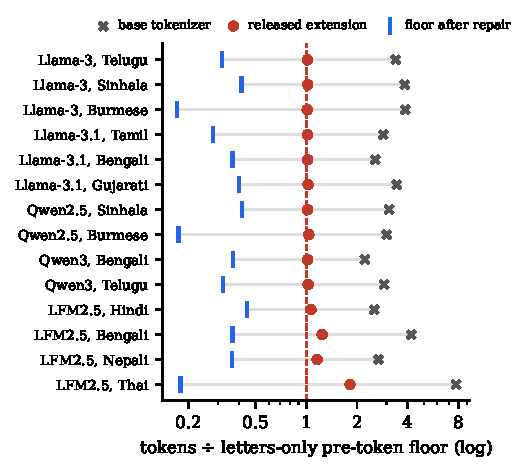
\includegraphics[width=0.95\columnwidth]{fig_released.pdf}
\caption{Released vocabulary extensions of letters-only models, on FLORES-200 devtest of each target language, relative to the letters-only pre-token floor. Ten extensions by \citet{yamaguchi2026lowres} (top) and LFM2.5~\citep{smith2026inplace} (bottom) move from the base tokenizer ($\times$) to the floor (\textcolor{red}{$\bullet$}) and stop there. The repaired regex would lower the floor to the blue tick. Full numbers, including the Amharic control, in Table~\ref{tab:released}.}
\label{fig:released}
\end{figure}